\section{Évaluation de l'hypothèse sur les coûts}
\label{section:4.3-HYPOTHESE-COUTS}
% : « \textit{combien dois-je investir ?} »

	%%% Formulation des hypothèses:
	Pour compléter l'étude réalisée sur l'hypothèse d'efficience (optimisation des paramètres de convergence, cf. section~\ref{section:4.2-HYPOTHESE-EFFICIENCE}), nous aimerions vérifier l'hypothèse suivante :
	\todo{à compléter}

	\begin{tcolorbox}[
		title=\faVial~\textbf{Hypothèse sur les coûts}~\faVial,
		colback=colorTcolorboxHypothesis!15,
		colframe=colorTcolorboxHypothesis!75,
		width=\linewidth
	]
		% Hypothèse.
		«\textbf{
			Il est possible d'\textbf{estimer les coûts nécessaires} d'une méthodologie d'annotation basée sur le \textit{clustering} interactif pour obtenir une base d'apprentissage exploitable. Nous étudierons en particulier les coûts relatifs au temps d'annotation, au temps de calculs des algorithmes, ainsi que la durée totale de la méthode en fonction de la taille du jeu de données.
		} » \\

		% Résumé de l'étude.
		Afin de vérifier cette hypothèse, nous organiserons plusieurs expériences pour simuler ou déterminer ces durées en fonction de plusieurs facteurs : taille du jeu de données, nombre de clusters, nombre de contraintes, différents annotateurs, ...
		
		% Figure.
		La figure~\ref{figure:4.3-HYPOTHESE-COUTS} illustre cette hypothèse et l'espoir de pouvoir caractériser la qualité de la base d'apprentissage en cours de construction en fonction d'un coût temporel au lieu d'un nombre abstrait d'itérations de la méthode. 
		%
		
		\begin{figure}[H]  % keep [H] to be in the tcolorbox.
			\centering
			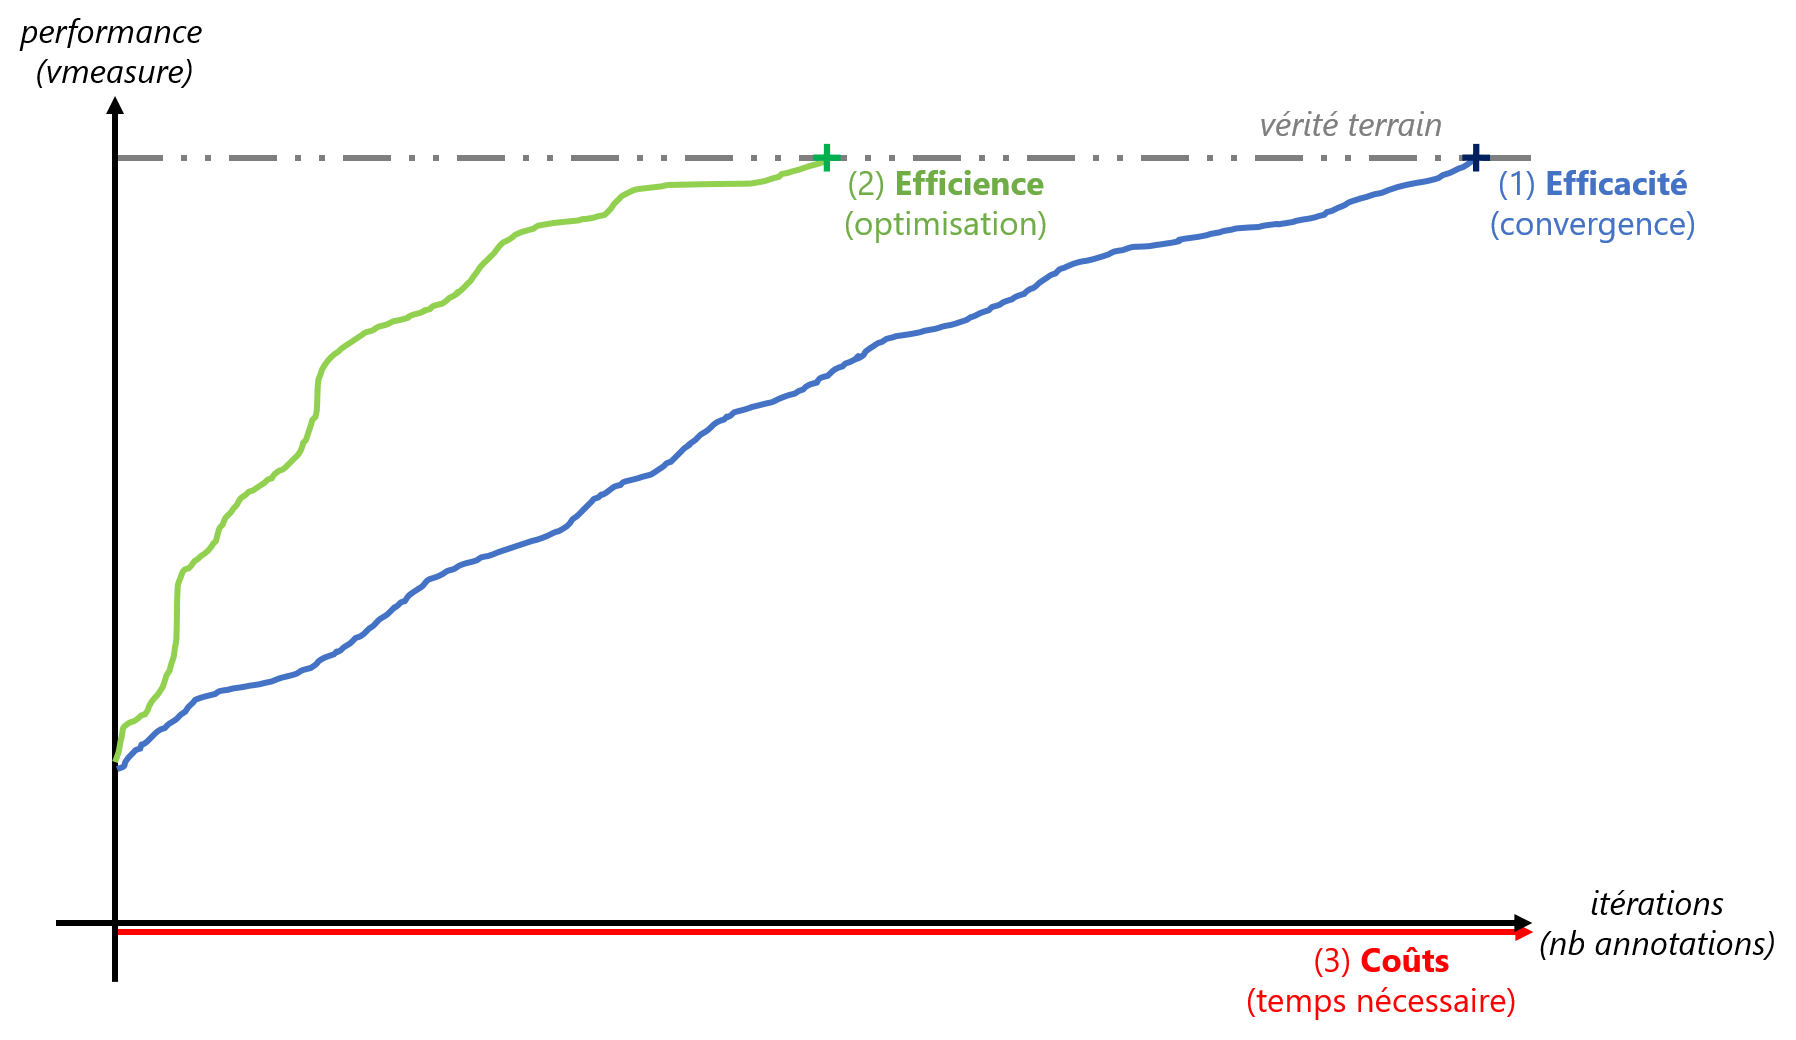
\includegraphics[width=0.8\textwidth]{figures/hypotheses-03-couts}
			\caption{Illustration des études réalisées sur le \textit{clustering} interactif (\textit{étape 3/6}) en schématisant l'évolution de la performance (\textit{accord avec la vérité terrain calculé en v-measure}) d'une base d'apprentissage en cours de construction en fonction du nombre d'itérations de la méthode (\textit{nombre d'annotations par un expert métier}).}
			\label{figure:4.3-HYPOTHESE-COUTS}
		\end{figure}

	\end{tcolorbox}
	

	%%%
	%%% Subsection 4.3.1: Étude du temps de calcul des algorithmes
	%%%
	\subsection{Étude du temps de calcul des algorithmes}
	\label{section:4.3.1-ETUDE-COUTS-TEMPS-CALCUL}
	
		%%% Protocole expérimental.
		\subsubsection{Protocole expérimental : estimer le temps de calcul des algorithmes du \textit{clustering} interactif}
		
			% Objectif de l'expérience.
			Pour confirmer le choix du paramétrage pour une convergence optimale (cf. hypothèse d'efficience en section~\ref{section:4.2-HYPOTHESE-EFFICIENCE}), nous voulons étudier le temps de calcul de chaque algorithme intervenant dans notre implémentation du \textit{clustering} interactif.
			Pour cela, nous allons chronométrer plusieurs exécutions de ces algorithmes avec différents paramètres d'entrée (la taille du jeu de données, le nombre de clusters et le nombre de contraintes annotées, ...) et modéliser le temps de calcul résultant en fonction de ces paramètres.
			
			% Remarques.
			\begin{leftBarWarning}
				Pour utiliser des jeux de données de tailles différentes tout en maîtrisant leur contenu, nous avons dupliqués aléatoirement des données en générant des fautes de frappes. Pour cette étude, nous faisons l'hypothèse que cela n'a pas d'impact majeur sur le temps d'exécution des différents algorithmes.
			\end{leftBarWarning}
			
			% Pseudo-code.
			Pour résumer le protocole expérimental que nous décrivons c-dessous, vous pouvez vous référer aux pseudo-code décrit dans Alg.~\ref{algorithm:4.3.1-ETUDE-COUTS-TEMPS-CALCUL-PROTOCOLE}.
			%
			\begin{algorithm}[!htb]
				\begin{algorithmic}[1]
					\ForAll{arrangement d'algorithmes et de paramètres à tester}
						\State \textbf{initialisation}: récupérer ou générer le jeu de données
						\If{estimation de la tâche de \textbf{prétraitement}}
							\State \textbf{chronomètre: START}
							\State \textbf{prétraitement}: supprimer le bruit dans les données
							\State \textbf{chronomètre: STOP}
						\ElsIf {estimation de la tâche de \textbf{vectorisation}}
							\State \textbf{prétraitement}: supprimer le bruit dans les données
							\State \textbf{chronomètre: START}
							\State \textbf{vectorisation}: transformer les données en vecteurs
							\State \textbf{chronomètre: STOP}
						\ElsIf {estimation de la tâche de \textbf{clustering}}
							\State \textbf{prétraitement}: supprimer le bruit dans les données
							\State \textbf{vectorisation}: transformer les données en vecteurs
							\State \textbf{échantillonnage initial}: sélectionner une base de contraintes à annoter
							\State \textbf{chronomètre: START}
							\State \textbf{clustering}: regrouper les données par similarité avec les contraintes
							\State \textbf{chronomètre: STOP}
						\ElsIf {estimation de la tâche d'\textbf{échantillonnage}}
							\State \textbf{prétraitement}: supprimer le bruit dans les données
							\State \textbf{vectorisation}: transformer les données en vecteurs
							\State \textbf{échantillonnage initial}: sélectionner une base de contraintes à annoter
							\State \textbf{clustering initial}: regrouper les données par similarité avec les contraintes
							\State \textbf{chronomètre: START}
							\State \textbf{échantillonnage}: sélectionner de nouvelles contraintes à annoter
							\State \textbf{chronomètre: STOP}
						\EndIf
						\State \textbf{mesure}: estimer la différence de chronomètre
					\EndFor
					\ForAll{algorithme à modéliser}
						\State \textbf{cadrage}: définir les facteurs et les interactions intervenant dans la modélisation
						\State \textbf{simplification}: restreindre la modélisation aux facteurs les plus corrélés
						\State \textbf{modélisation}: entraîner un modèle linéaire généralisé avec les facteurs retenus
						\State \textbf{simulation}: écrire l'équation du temps d'exécution avec des paramètres obtenus
					\EndFor
					\Ensure modélisation du temps d'exécution des différents algorithmes
				\end{algorithmic}
				\caption{Description en pseudo-code du protocole expérimental de modélisation du temps d'exécution des algorithmes du \textit{clustering} interactif}
				\label{algorithm:4.3.1-ETUDE-COUTS-TEMPS-CALCUL-PROTOCOLE}
			\end{algorithm}
			
			% Description des tâches, des algorithmes et des paramètres.
			Pour cette étude, nous lançons plusieurs exécutions de chaque algorithme de notre implémentation du clustering interactif (cf. section~\ref{section:3.3-DESCRIPTION-IMPLEMENTATION}) avec différents variations de données d'entrée. Cela comprend les tâches, algorithmes et données d'entrée suivants :
			%
			\begin{enumerate}
				% Prétraitement.
				\item le \textbf{prétraitement} des données...
					\begin{itemize}
						\item avec les algorithmes suivants : \textbf{simple} (noté \texttt{prep.simple}), \textbf{avec lemmatisation} (noté \texttt{prep.lemma}) et \textbf{avec filtres} (noté \texttt{prep.filter}) ;
						\item avec les données d'entrée suivantes : \textbf{nombre de données} (variant de $1~000$ à $5~000$ par pas de $1~000$, noté $\texttt{dataset\_size}$) ;
					\end{itemize}
				% Vectorisation.
				\item la \textbf{vectorisation} des données...
					\begin{itemize}
						\item avec les algorithmes suivants : \textbf{TF-IDF} (noté \texttt{vect.tfidf}) et \textbf{SpaCy} (noté \texttt{vect.frcorenewsmd}) ;
						\item avec les données d'entrée suivantes : \textbf{nombre de données} (variant de $1~000$ à $5~000$ par pas de $1~000$, noté $\texttt{dataset\_size}$) ;
						\item précédé par un prétraitement \textbf{simple} ;
					\end{itemize}
				% Clustering.
				\item le \textbf{clustering sous contraintes} des données...
					\begin{itemize}
						\item avec les algorithmes suivants : \textbf{KMeans} (modèle \textit{COP} noté \texttt{clust.kmeans.cop}), \textbf{Hiérarchique} (lien \textit{single} noté \texttt{clust.hier.sing} ; lien \textit{complete} noté \texttt{clust.hier.comp} ; lien \textit{average} noté \texttt{clust.hier.avg} ; lien \textit{ward} noté \texttt{clust.hier.ward}) et \textbf{Spectral} (modèle \textit{SPEC} noté \texttt{clust.spec}) ;
						\item avec les données d'entrée suivantes : \textbf{nombre de données} (variant de $1~000$ à $5~000$ par pas de $1~000$, noté $\texttt{dataset\_size}$), le \textbf{nombre de contraintes annotés} (variant de $0$ à $5~000$ par pas de $500$, noté $\texttt{previous\_nb\_constraints}$) et le \textbf{nombre de \textit{clusters} à trouver} (variant de $5$ à $50$ par pas de $5$, noté $\texttt{algorithm\_nb\_clusters}$) ;
						\item précédé par un prétraitement \textbf{simple} et une vectorisation \textbf{TF-IDF} et un échantillonnage initial \textbf{purement aléatoire} ;
					\end{itemize}
				% Sampling.
				\item l'\textbf{échantillonnage} des contraintes à annoter...
					\begin{itemize}
						\item avec les algorithmes suivants : \textbf{purement aléatoire} (noté \texttt{samp.random.full}), \textbf{pseudo-aléatoire} (noté \texttt{samp.random.same}), \textbf{même cluster et étant les plus éloignées} (noté \texttt{samp.farhtest.same}) et \textbf{clusters différents et étant les plus proches} (noté \texttt{samp.closest.diff}) ;
						\item avec les données d'entrée suivantes : \textbf{nombre de données} (variant de $1~000$ à $5~000$ par pas de $1~000$, noté $\texttt{dataset\_size}$), le \textbf{nombre de contraintes annotés} (variant de $0$ à $5~000$ par pas de $500$, noté $\texttt{previous\_nb\_constraints}$), le \textbf{nombre de \textit{clusters} existant} (variant de $10$ à $50$ par pas de $10$, noté $\texttt{previous\_nb\_clusters}$) et le \textbf{nombre de contraintes à sélectionner} (variant de $50$ à $250$ par pas de $50$, noté $\texttt{algorithm\_nb\_constraints}$) ;
						\item précédé par un prétraitement \textbf{simple}, une vectorisation \textbf{TF-IDF}, un \textit{clustering} initial \textbf{KMeans} (modèle \textit{COP}) et un échantillonnage initial \textbf{purement aléatoire} ;
					\end{itemize}
			\end{enumerate}
			
			Il y a donc $8~825$ combinaisons d'algorithmes (\texttt{15} pour le prétraitement, $10$ pour la vectorisation, $3~330$ pour le \textit{clustering}, $5~550$ pour l'échantillonnage), et chaque combinaison est répétée $5$ fois pour contrer les aléas statistiques des exécutions.
			De plus, chaque jeu de données est généré $5$ fois pour contrer les aléas statistiques de création, donc il y a $220~625$ exécutions d'algorithmes ($375$ pour le prétraitement, $250$ pour la vectorisation, $82~500$ pour le \textit{clustering}, $137~500$ pour l'échantillonnage).
			
			% Description de la modélisation.
			Sur la base de ces mesures, nous cherchons à modéliser le temps d'exécution de chaque algorithme en fonction de ses paramètres d'entrée\footnote{Les paramètres d'entrée peuvent être : le nombre de données, le nombre de contraintes annotées, le nombre de contraintes à sélectionner, le nombre de \textit{clusters} existant, le nombre de \textit{clusters} à trouver}, et les interactions doubles entre paramètres sont envisagées.
			Afin de réduire la complexité des modélisations, nous ordonnons les interactions de facteurs possibles en fonction de leur corrélation avec le temps mesuré (la corrélation \texttt{r} de \textit{Pearson} est utilisée) et nous nous limitons aux variables responsables d'un maximum de la variance des mesures (la méthode d'\textit{Elbow} est utilisée pour choisir les facteurs pertinents).
			Sur cette base, nous entraînons un modèle linéaire généralisé (\textit{GLM}) pour représenter le temps d'exécution de l'algorithme : ce modèle sera caractérisé par le coefficient de détermination généralisé \texttt{R²} de \textit{Cox et Snel}, la log-vraisemblance \texttt{llf} et la log-vraisemblance \texttt{llf\_null} du modèle \textit{null}.
			Pour finir, nous discuterons des valeurs des coefficients obtenus sur l'impact du temps d'exécution.
			Ces analyses sont réalisées en Python\todo{citation} à l'aide des librairies \texttt{datetime}\todo{citation} et \texttt{statsmodels} (\cite{seabold:2010}).
			
			% Référence scripts.
			\begin{leftBarInformation}
				Les scripts de l'expérience (\textit{notebooks} Python) sont disponibles dans un dossier dédié de~\cite{schild:cognitivefactory-interactive-clustering-comparative-study:2021}.
			\end{leftBarInformation}

		%%% Résultats
		\subsubsection{Résultats obtenus}
				
			%%% Prétraitements
			
			% Première analyse.
			En ce qui concerne la tâche de \textbf{prétraitement}, une première analyse montre que les modélisations des trois implémentations sont similaires  (\texttt{p-valeur}: $> 0.980$). Nous ferons donc une seule modélisation.
			
			% Modélisation du temps de calcul (prep.simple + prep.lemma + prep.filter).
			Pour les algorithmes de prétraitements (\texttt{prep.simple}, \texttt{prep.lemma} et \texttt{prep.filter}), l'analyse de la corrélation des facteurs avec les mesures de temps d'exécution indique qu'une modélisation minimale et suffisante peut être réalisée à partir du facteur $\texttt{dataset\_size}$ (\texttt{r}: $0.997$).
			Le modèle linéaire généralisé retenu (\texttt{R²}: $> 0.999$, \texttt{llf}: $-379.35$, \texttt{llf\_null}: $-1~353.98$) nous permet de déduire l'équation suivante\footnote{Cette déduction est en accord avec la complexité théorique de l'algorithme qui est en $ \mathcal{O}(\texttt{dataset\_size}) $.}\todo{ref annexe} :
			%
			\begin{equation}
				time(prep)
				\simeq 8.39\cdot10^{-1} + 6.31\cdot10^{-3}\cdot\texttt{dataset\_size}
			\end{equation}
			
			% Affichage du temps de calcul.
			La figure~\ref{figure:4.3.1-ETUDE-COUTS-TEMPS-CALCUL-MODELISATION-PREPROCESSING} représente cette simulation du temps de calcul des algorithmes de prétraitements en comparaison avec les mesures réalisées lors de l'expérience.
			\newline
			%		
			\begin{figure}[!htb]
				\centering
				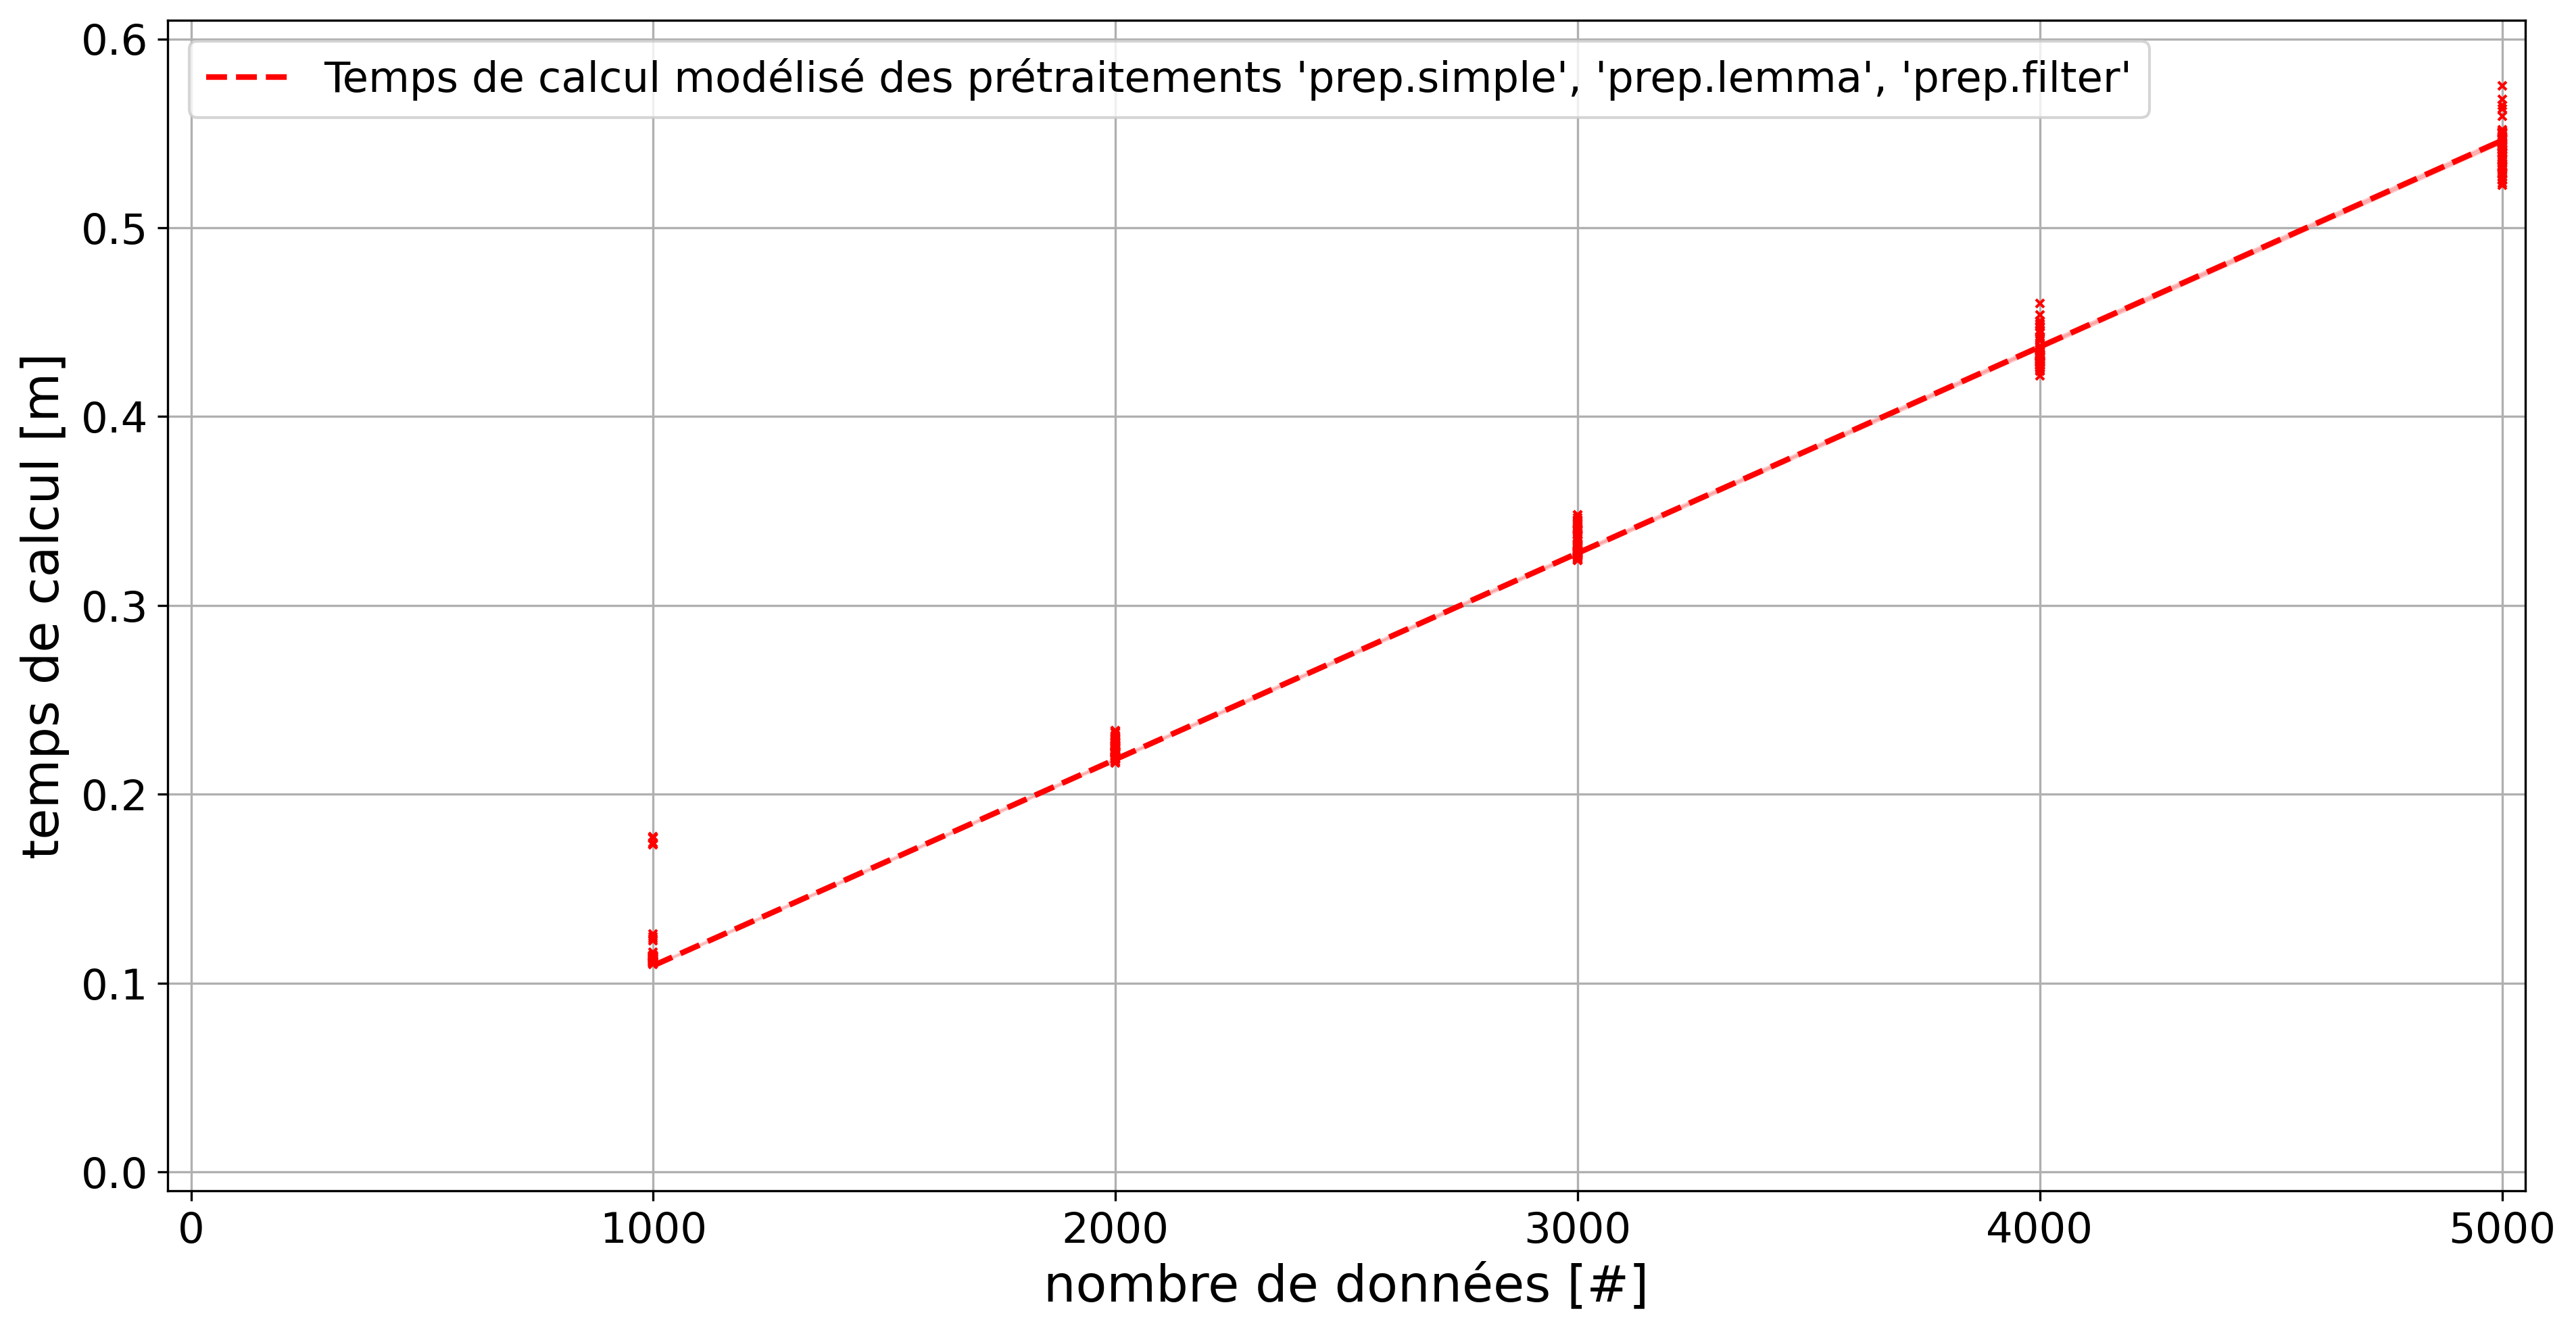
\includegraphics[width=0.8\textwidth]{figures/etude-temps-calcul-modelisation-1prep}
				\caption{Estimation du temps nécessaire (en secondes) pour effectuer une tâche de \textbf{prétraitement} en fonction du nombre de données à traiter. Les paramétrages \texttt{prep.simple}, \texttt{prep.lemma} et \texttt{prep.filter} ayant des temps de calculs similaires, leurs modélisations n'ont pas été séparées.}
				\label{figure:4.3.1-ETUDE-COUTS-TEMPS-CALCUL-MODELISATION-PREPROCESSING}
			\end{figure}
			
			%%% Vectorization
			
			% Première analyse.
			En ce qui concerne la tâche de \textbf{vectorisation}, une première analyse montre que les modélisations des deux implémentations sont différentiables  (\texttt{p-valeur}: $< 10^{-3}$). Nous ferons donc une modélisation par algorithme.
		
			% Modélisation du temps de calcul (vect.tfidf).
			Pour les algorithmes de vectorisation \texttt{vect.tfidf}, l'analyse de la corrélation des facteurs avec les mesures de temps d'exécution indique qu'une modélisation minimale et suffisante peut être réalisée à partir du facteur $\texttt{dataset\_size}$ (\texttt{r}: $0.977$).
			Le modèle linéaire généralisé retenu (\texttt{R²}: $> 0.999$, \texttt{llf}: $262.35$, \texttt{llf\_null}: $70.04$) nous permet de déduire l'équation suivante\footnote{Cette déduction est en accord avec la complexité théorique de l'algorithme qui est en $ \mathcal{O}(\texttt{dataset\_size}) $.}\todo{ref annexe} :
			%
			\begin{equation}
				time(vect.tfidf)
				\simeq -1.40\cdot10^{-2} + 9.54\cdot10^{-5}\cdot\texttt{dataset\_size}
			\end{equation}
			
			% Modélisation du temps de calcul (vect.frcorenewsmd).
			Pour les algorithmes de vectorisation \texttt{vect.frcorenewsmd}, l'analyse de la corrélation des facteurs avec les mesures de temps d'exécution indique qu'une modélisation minimale et suffisante peut être réalisée à partir du facteur $\texttt{dataset\_size}$ (r: $0.983$).
			Le modèle linéaire généralisé retenu (\texttt{R²}: $> 0.999$, \texttt{llf}: $-186.80$, \texttt{llf\_null}: $-399.39$) nous permet de déduire l'équation suivante\footnote{Cette déduction est en accord avec la complexité théorique de l'algorithme qui est en $ \mathcal{O}(\texttt{dataset\_size}) $.}\todo{ref annexe} :
			%
			\begin{equation}
				time(vect.frcorenewsmd)
				\simeq 1.89 + 4.11\cdot10^{-3}\cdot\texttt{dataset\_size}
			\end{equation}
			
			% Affichage du temps de calcul.
			La figure~\ref{figure:4.3.1-ETUDE-COUTS-TEMPS-CALCUL-MODELISATION-VECTORIZATION} représente ces simulations de temps de calcul des algorithmes de vectorisation en comparaison avec les mesures réalisées lors de l'expérience.
			\newline
			%
			\begin{figure}[!htb]
				\centering
				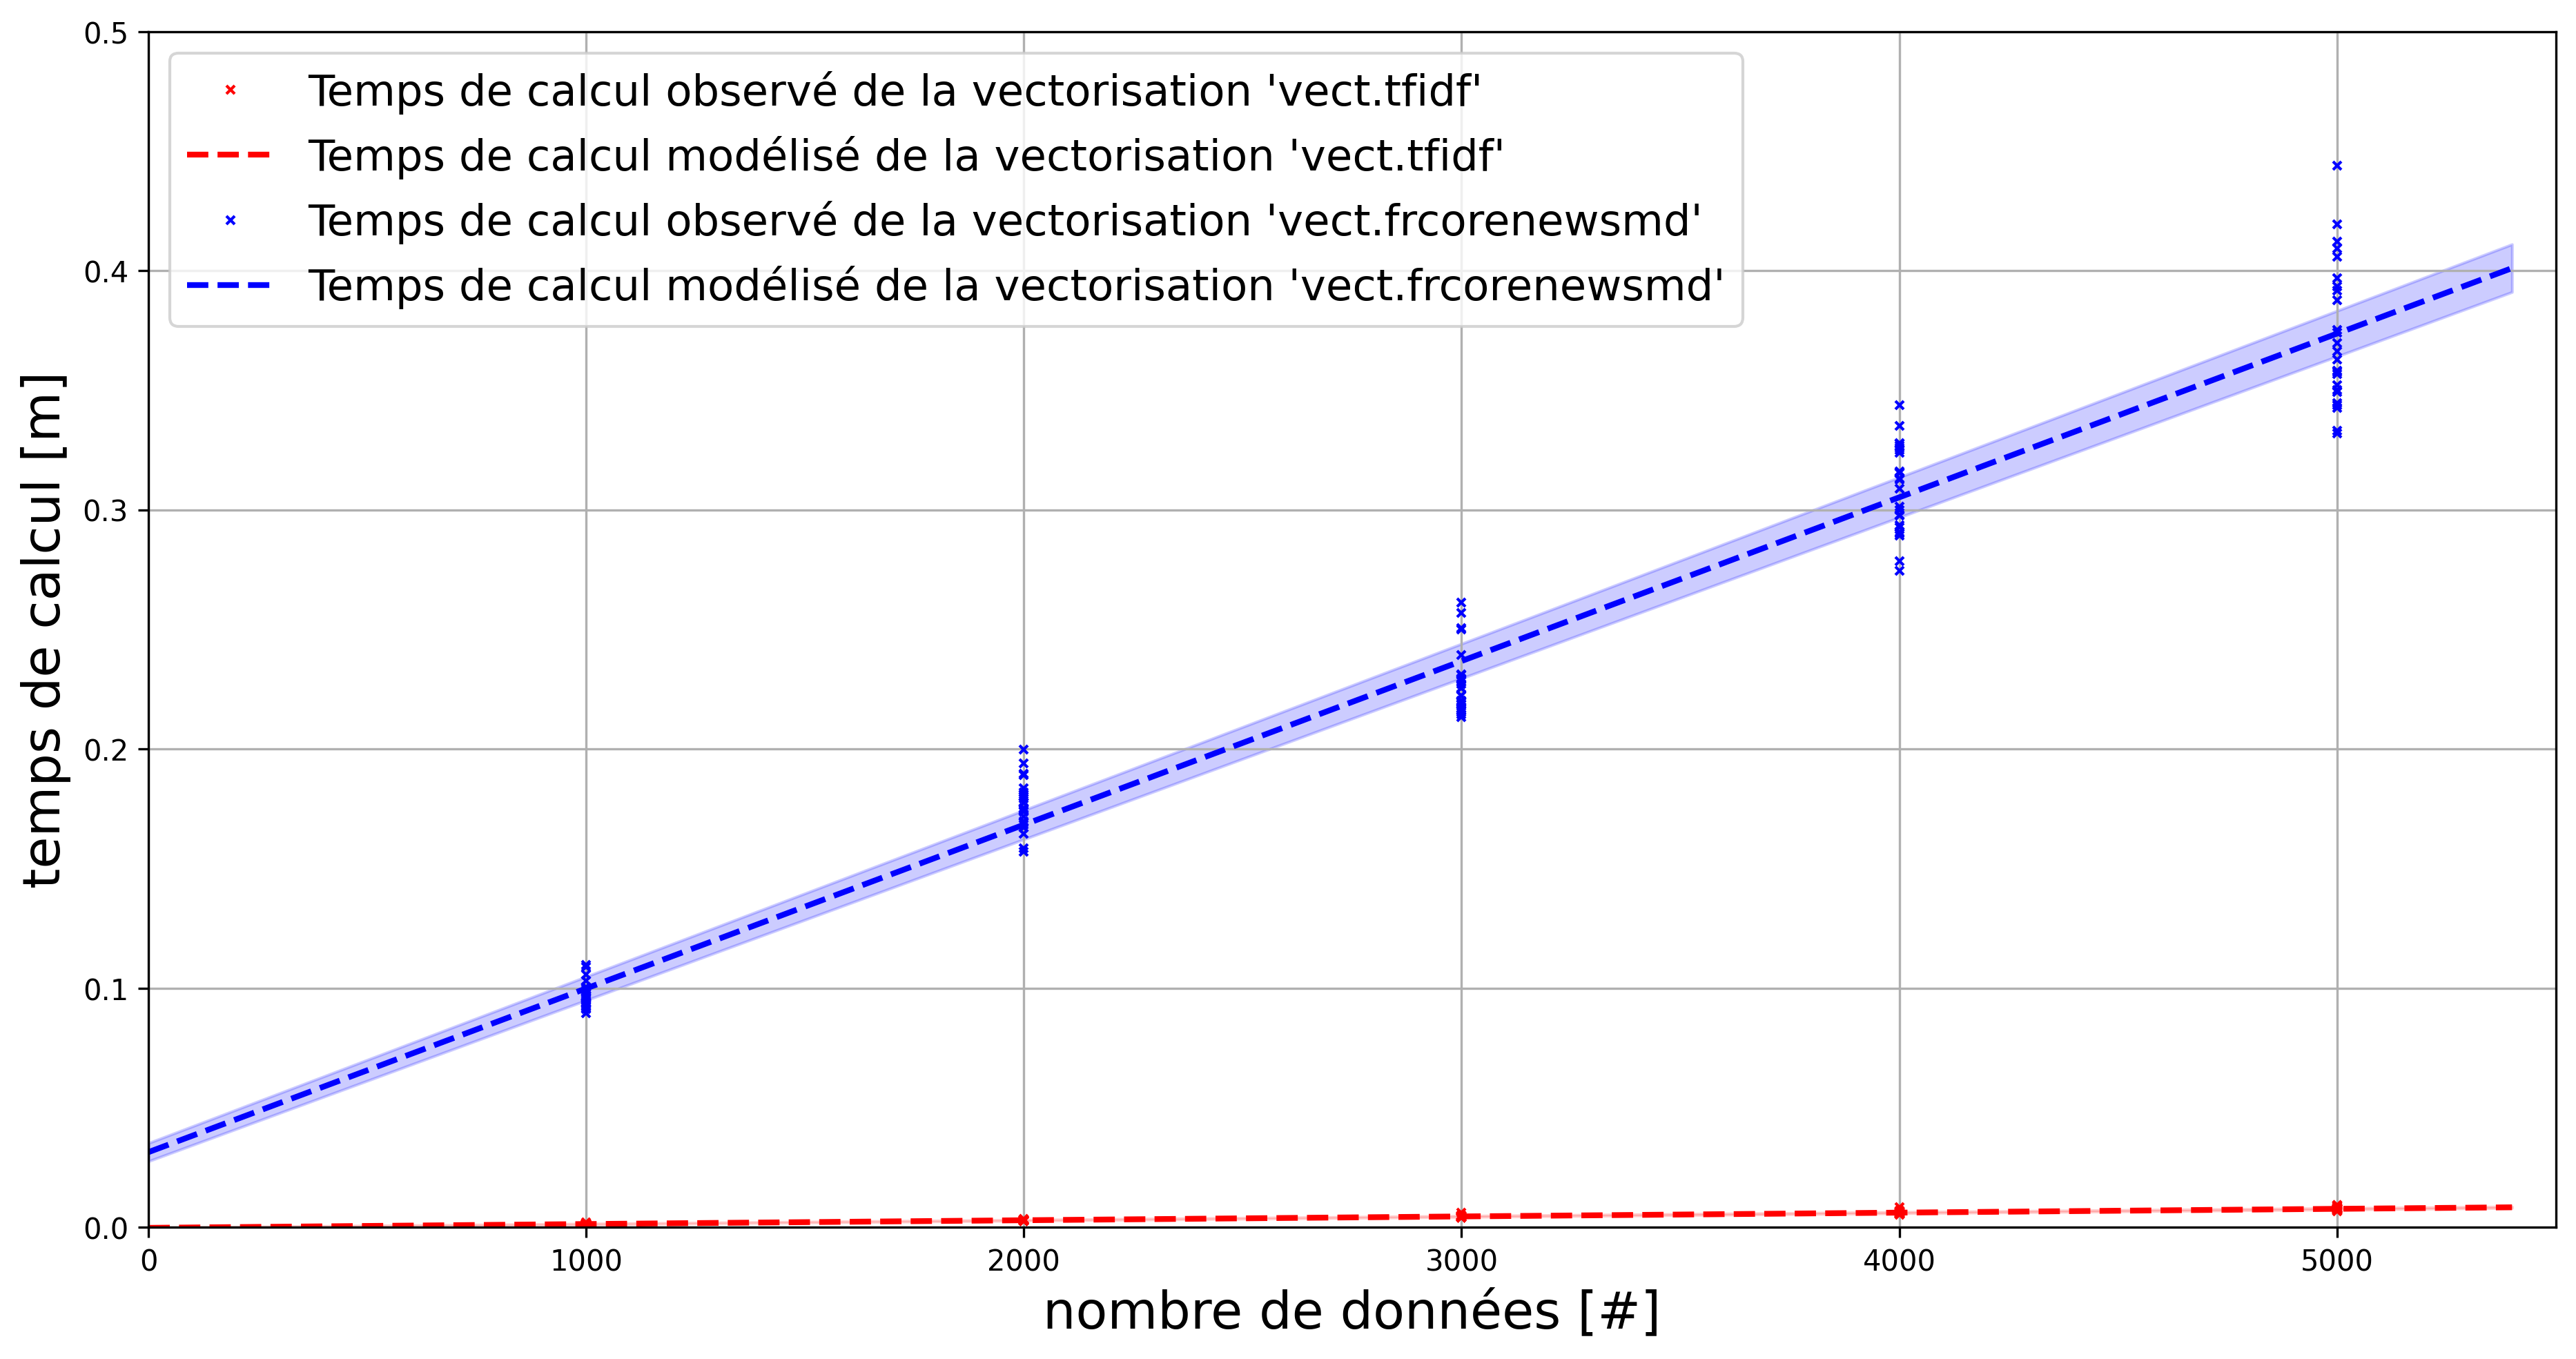
\includegraphics[width=0.8\textwidth]{figures/etude-temps-calcul-modelisation-2vect}
				\caption{Estimation du temps nécessaire (en secondes) pour effectuer une tâche de \textbf{vectorisation} en fonction du nombre de données à traiter.}
				\label{figure:4.3.1-ETUDE-COUTS-TEMPS-CALCUL-MODELISATION-VECTORIZATION}
			\end{figure}
			
			%%% Clustering
			
			% Première analyse.
			En ce qui concerne la tâche de \textbf{\textit{clustering} sous contraintes}, une première analyse montre que les modélisations des six implémentations sont différentiables  (\texttt{p-valeur}: $<$ \texttt{$10^{-3}$}). Nous ferons donc une modélisation par algorithme.
			
			% Modélisation du temps de calcul (clust.kmeans.cop).
			Pour les algorithmes du \textit{clustering} sous contraintes \texttt{clust.kmeans.cop}, l'analyse de la corrélation des facteurs avec les mesures de temps d'exécution indique qu'une modélisation minimale et suffisante peut être réalisée à partir du facteur $\texttt{dataset\_size}$ (r: $0.837$).
			Le second facteur le plus corrélé (mais non retenu) est l'interaction $(\texttt{dataset\_size})^{2}\cdot(algorithm\_nb\_clusters)$ (r: $0.545$).
			Le modèle linéaire généralisé retenu (\texttt{R²}: $0.904$, \texttt{llf}: $-9.20\cdot10^{4}$, \texttt{llf\_null}: $-1.00\cdot10^{5}$) nous permet de déduire l'équation suivante\todo{ref annexe} :
			%
			\begin{equation}
				time(clust.kmeans.cop)
				\simeq -2.40\cdot10^{-2} + 2.11\cdot10^{-1}\cdot\texttt{dataset\_size}
			\end{equation}
			
			% Modélisation du temps de calcul (clust.hier.sing).
			Pour les algorithmes du \textit{clustering} sous contraintes \texttt{clust.hier.sing}, l'analyse de la corrélation des facteurs avec les mesures de temps d'exécution indique qu'une modélisation minimale et suffisante peut être réalisée à partir du facteur $(\texttt{dataset\_size})^{2}$ (r: $0.940$).
			Le second facteur le plus corrélé (mais non retenu) est l'interaction $(\texttt{dataset\_size})^{2}\cdot(algorithm\_nb\_clusters)$ (r: $0.729$).
			Le modèle linéaire généralisé retenu (\texttt{R²}: $> 0.999$, \texttt{llf}: $-5.38\cdot10^{4}$, \texttt{llf\_null}: $-6.10\cdot10^{4}$) nous permet de déduire l'équation suivante\todo{ref annexe} :
			%
			\begin{equation}
				time(clust.hier.sing)
				\simeq -8.87\cdot10^{2} + 6.37\cdot10^{4}\cdot(\texttt{dataset\_size})^{2}
			\end{equation}
			
			% Modélisation du temps de calcul (clust.hier.comp).
			Pour les algorithmes du \textit{clustering} sous contraintes \texttt{clust.hier.comp}, l'analyse de la corrélation des facteurs avec les mesures de temps d'exécution indique qu'une modélisation minimale et suffisante peut être réalisée à partir du facteur $(\texttt{(dataset\_size})^{2}$ (r: $0.938$).
			Le second facteur le plus corrélé (mais non retenu) est l'interaction $(\texttt{dataset\_size})^{2}\cdot(algorithm\_nb\_clusters)$ (r: $0.736$).
			Le modèle linéaire généralisé retenu (\texttt{R²}: $> 0.999$, \texttt{llf}: $-5.40\cdot10^{4}$, \texttt{llf\_null}: $-6.11\cdot10^{4}$) nous permet de déduire l'équation suivante\todo{ref annexe} :
			%
			\begin{equation}
				time(clust.hier.comp)
				\simeq -9.25\cdot10^{2} + 6.42\cdot10^{4}\cdot(\texttt{dataset\_size})^{2}
			\end{equation}

			% Modélisation du temps de calcul (clust.hier.avg).
			Pour les algorithmes du \textit{clustering} sous contraintes \texttt{clust.hier.avg}, l'analyse de la corrélation des facteurs avec les mesures de temps d'exécution indique qu'une modélisation minimale et suffisante peut être réalisée à partir du facteur $(\texttt{(dataset\_size})^{2}$ (r: $0.915$).
			Le second facteur le plus corrélé (mais non retenu) est l'interaction $(\texttt{dataset\_size})^{2}\cdot(algorithm\_nb\_clusters)$ (r: $0.713$).
			Le modèle linéaire généralisé retenu (\texttt{R²}: $0.942$, \texttt{llf}: $-5.82\cdot10^{4}$, \texttt{llf\_null}: $-6.45\cdot10^{4}$) nous permet de déduire l'équation suivante\todo{ref annexe} :
			%
			\begin{equation}
				time(clust.hier.avg)
				\simeq -1.10\cdot10^{3} + 1.02\cdot10^{3}\cdot(\texttt{dataset\_size})^{2}
			\end{equation}

			% Modélisation du temps de calcul (clust.hier.ward).
			Pour les algorithmes du \textit{clustering} sous contraintes \texttt{clust.hier.ward}, l'analyse de la corrélation des facteurs avec les mesures de temps d'exécution indique qu'une modélisation minimale et suffisante peut être réalisée à partir du facteur $(\texttt{(dataset\_size})^{2}$ (r: $0.945$).
			Le second facteur le plus corrélé (mais non retenu) est l'interaction $(\texttt{dataset\_size})^{2}\cdot(algorithm\_nb\_clusters)$ (r: $0.734$).
			Le modèle linéaire généralisé retenu (\texttt{R²}: $> 0.999$, \texttt{llf}: $-5.39\cdot10^{4}$, \texttt{llf\_null}: $-6.14\cdot10^{4}$) nous permet de déduire l'équation suivante\todo{ref annexe} :
			%
			\begin{equation}
				time(clust.hier.ward)
				\simeq -9.79\cdot10^{2} + 6.82\cdot10^{4}\cdot(\texttt{dataset\_size})^{2}
			\end{equation}
			
			% Modélisation du temps de calcul (clust.spec).
			Pour les algorithmes du \textit{clustering} sous contraintes \texttt{clust.spec}, l'analyse de la corrélation des facteurs avec les mesures de temps d'exécution indique qu'une modélisation minimale et suffisante peut être réalisée à partir du facteur $(\texttt{(dataset\_size})^{2}$ (r: $0.658$).
			Le second facteur le plus corrélé (mais non retenu) est l'interaction $(\texttt{dataset\_size})^{2}\cdot(algorithm\_nb\_clusters)$ (r: $0.595$).
			Le modèle linéaire généralisé retenu (\texttt{R²}: $0.534$, \texttt{llf}: $-7.88\cdot10^{5}$, \texttt{llf\_null}: $-8.27\cdot10^{5}$) nous permet de déduire l'équation suivante\todo{ref annexe} :
			%
			\begin{equation}
				time(clust.spec)
				\simeq 11.00 + 7.56\cdot10^{-6}\cdot(\texttt{dataset\_size})^{2}
			\end{equation}
			
			% Affichage du temps de calcul.
			La figure~\ref{figure:4.3.1-ETUDE-COUTS-TEMPS-CALCUL-MODELISATION-CLUSTERING} représente ces simulations de temps de calcul des algorithmes de \textit{clustering} en comparaison avec les mesures réalisées lors de l'expérience.
			\newline
			%
			\begin{figure}[!htb]
				\centering
				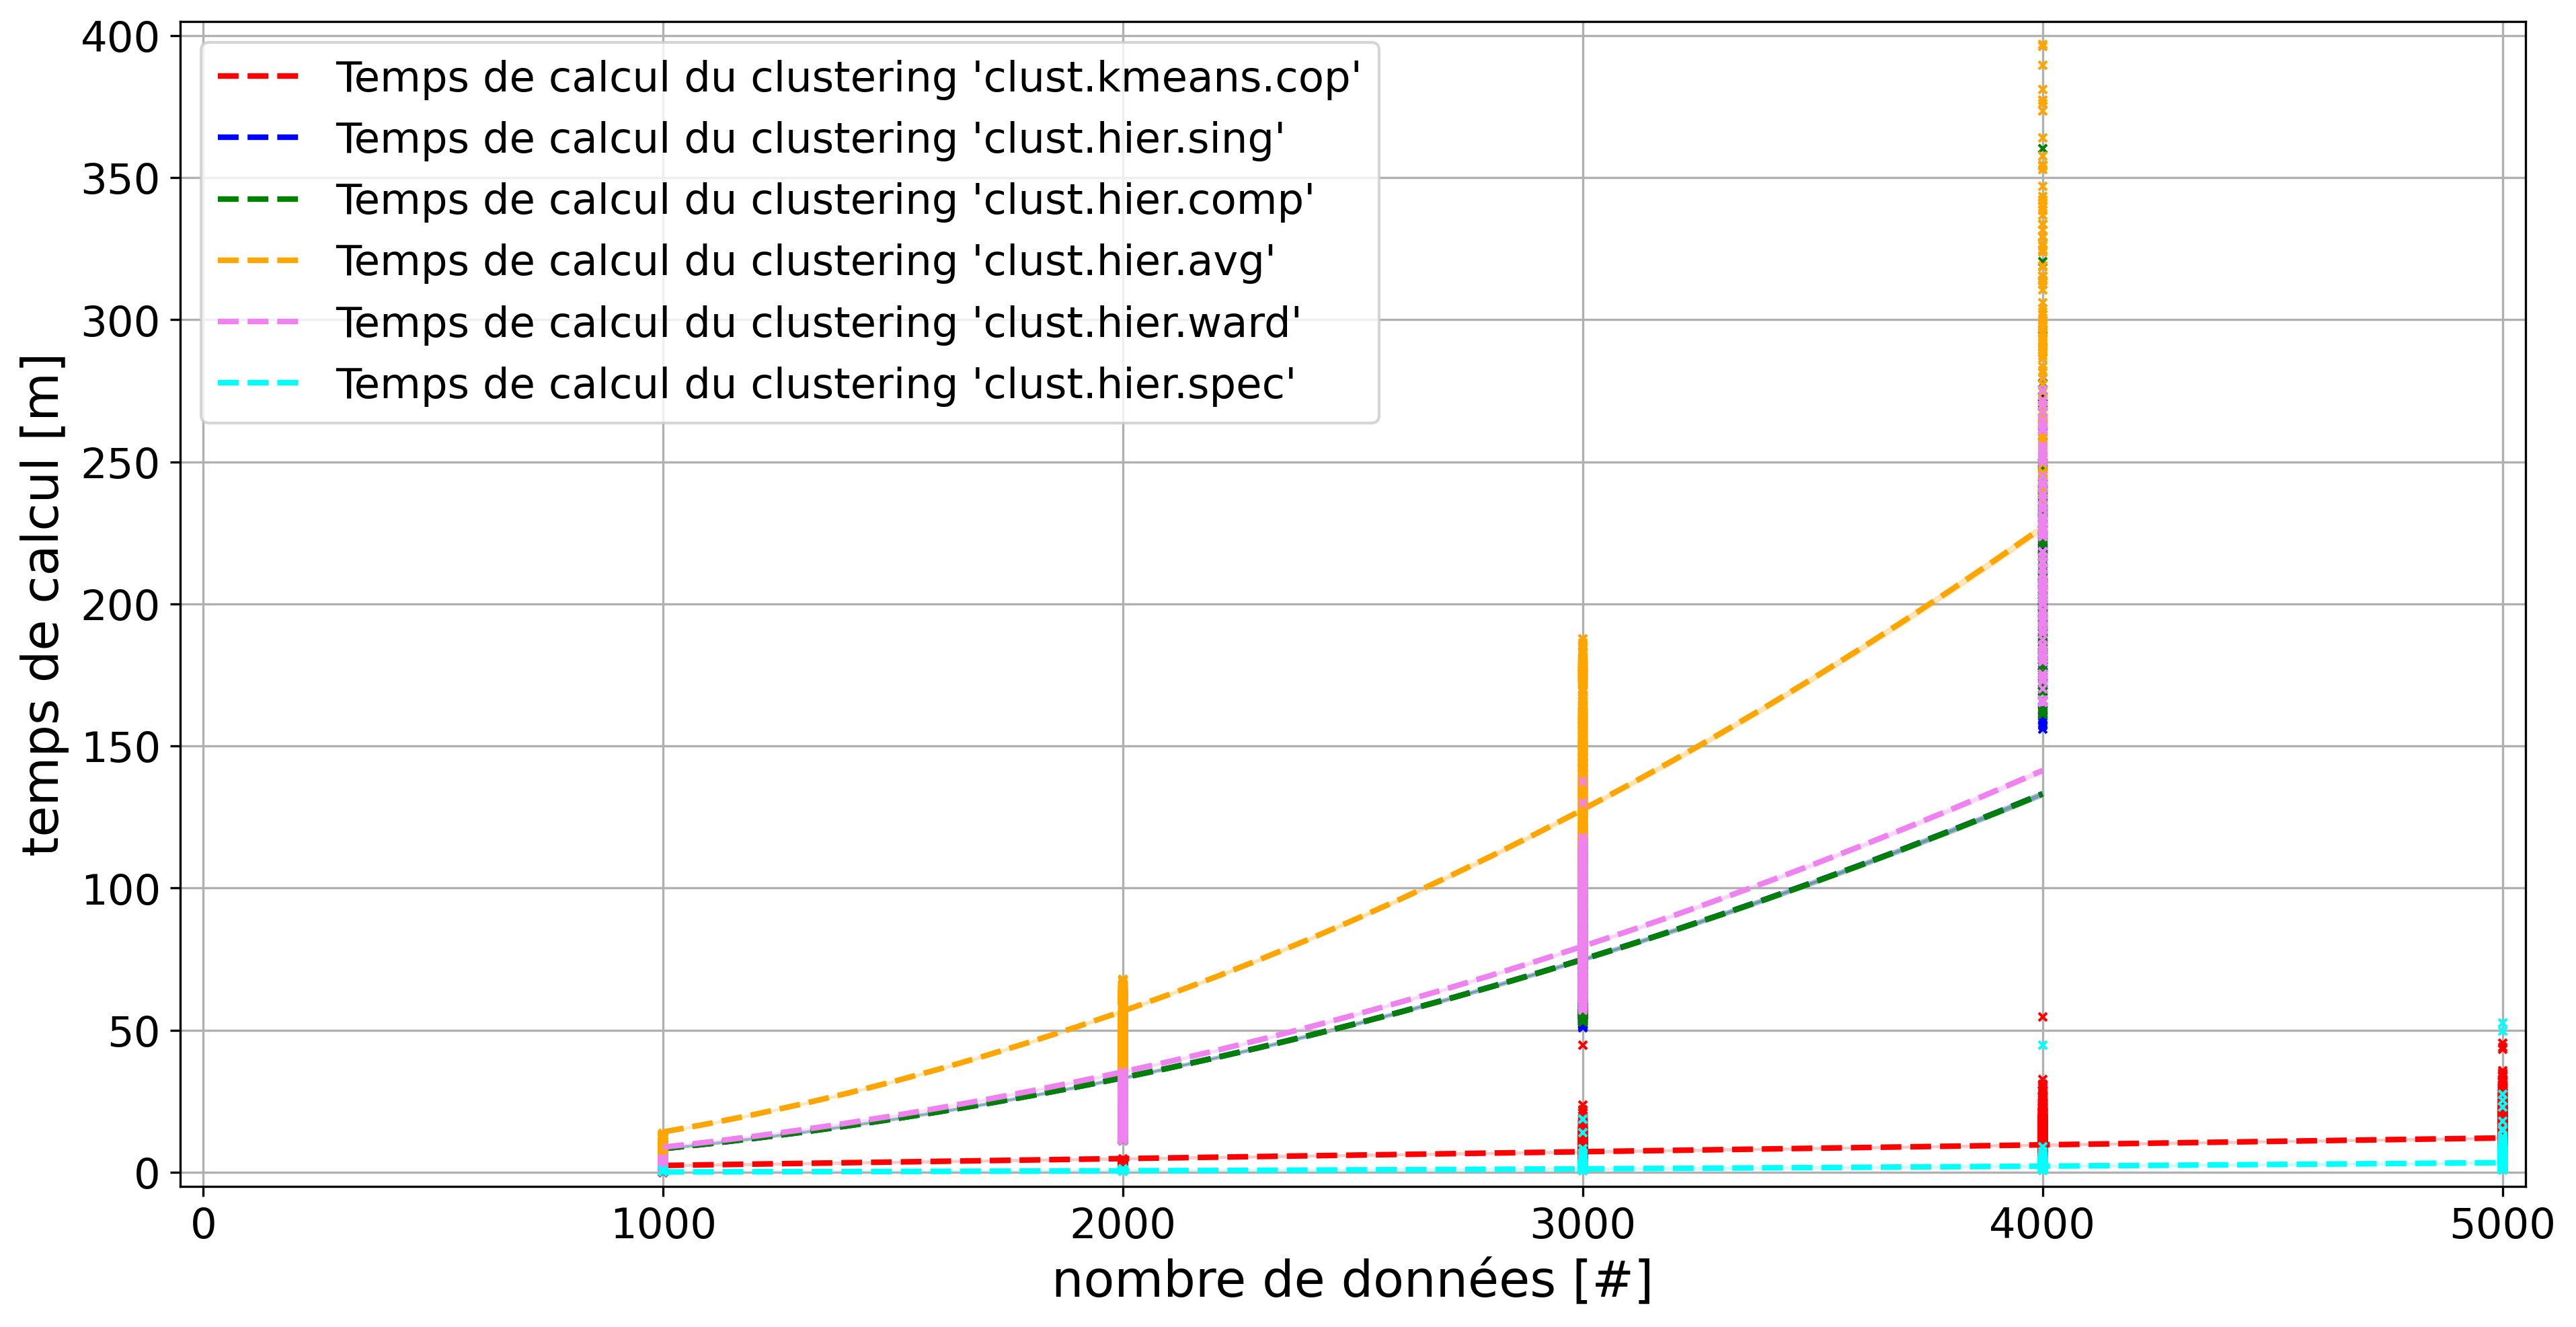
\includegraphics[width=0.8\textwidth]{figures/etude-temps-calcul-modelisation-3clust}
				\caption{Estimation du temps nécessaire (en secondes) pour effectuer une tâche de \textbf{clustering} en fonction du nombre de données à traiter.}
				\label{figure:4.3.1-ETUDE-COUTS-TEMPS-CALCUL-MODELISATION-CLUSTERING}
			\end{figure}
			
			%%% Sampling
			
			% Première analyse.
			En ce qui concerne la tâche d'\textbf{échantillonnage de contraintes}, une première analyse montre que les modélisations des quatre implémentations sont différentiables  (\texttt{p-valeur}: $<$ \texttt{$10^{-3}$}). Nous ferons donc une modélisation par algorithme.
			
			% Modélisation du temps de calcul (samp.rand.full).
			Pour les algorithmes de l'échantillonnage de contraintes \texttt{samp.rand.full}, l'analyse de la corrélation des facteurs avec les mesures de temps d'exécution indique qu'une modélisation minimale et suffisante peut être réalisée à partir du facteur $(\texttt{dataset\_size})^{2}$ (r: $0.993$).
			Le second facteur le plus corrélé (mais non retenu) est l'interaction $(\texttt{dataset\_size})^{2}\cdot(previous\_nb\_clusters)$ (r: $0.791$).
			Le modèle linéaire généralisé retenu (\texttt{R²}: $> 0.999$, \texttt{llf}: $-4.33\cdot10^{4}$, \texttt{llf\_null}: $-1.17\cdot10^{5}$) nous permet de déduire l'équation suivante\todo{ref annexe} :
			%
			\begin{equation}
				time(clust.kmeans.cop)
				\simeq -4.78\cdot10^{-1} + 8.47\cdot10^{-7}\cdot(\texttt{dataset\_size})^{2}
			\end{equation}
			
			% Modélisation du temps de calcul (samp.rand.same).
			Pour les algorithmes de l'échantillonnage de contraintes \texttt{samp.rand.same}, l'analyse de la corrélation des facteurs avec les mesures de temps d'exécution indique qu'une modélisation minimale et suffisante peut être réalisée à partir du facteur $(\texttt{dataset\_size})^{2}$ (r: $0.939$).
			Le second facteur le plus corrélé (mais non retenu) est l'interaction $(\texttt{dataset\_size})^{2}\cdot(algorithm\_nb\_constraints)$ (r: $0.611$).
			Le modèle linéaire généralisé retenu (\texttt{R²}: $> 0.999$, \texttt{llf}: $-3.17\cdot10^{4}$, \texttt{llf\_null}: $-6.84\cdot10^{4}$) nous permet de déduire l'équation suivante\todo{ref annexe} :
			%
			\begin{equation}
				time(clust.kmeans.cop)
				\simeq -1.36\cdot10^{-1} + 1.92\cdot10^{-7}\cdot(\texttt{dataset\_size})^{2}
			\end{equation}
			
			% Modélisation du temps de calcul (samp.farhtest.same).
			Pour les algorithmes de l'échantillonnage de contraintes \texttt{samp.farhtest.same}, l'analyse de la corrélation des facteurs avec les mesures de temps d'exécution indique qu'une modélisation minimale et suffisante peut être réalisée à partir du facteur $(\texttt{dataset\_size})^{2}$ (r: $0.981$).
			Le second facteur le plus corrélé (mais non retenu) est l'interaction $(\texttt{dataset\_size})^{2}\cdot(previous\_nb\_clusters)$ (r: $0.700$).
			Le modèle linéaire généralisé retenu (\texttt{R²}: $> 0.999$, \texttt{llf}: $-4.52\cdot10^{4}$, \texttt{llf\_null}: $-1.02\cdot10^{5}$) nous permet de déduire l'équation suivante\todo{ref annexe} :
			%
			\begin{equation}
				time(clust.kmeans.cop)
				\simeq -2.25\cdot10^{-1} + 5.32\cdot10^{-7}\cdot(\texttt{dataset\_size})^{2}
			\end{equation}
			
			% Modélisation du temps de calcul (samp.closest.diff).
			Pour les algorithmes de l'échantillonnage de contraintes \texttt{samp.closest.diff}, l'analyse de la corrélation des facteurs avec les mesures de temps d'exécution indique qu'une modélisation minimale et suffisante peut être réalisée à partir du facteur $(\texttt{dataset\_size})^{2}$ (r: $0.995$).
			Le second facteur le plus corrélé (mais non retenu) est l'interaction $(\texttt{dataset\_size})^{2}\cdot(previous\_nb\_clusters)$ (r: $0.815$).
			Le modèle linéaire généralisé retenu (\texttt{R²}: $> 0.999$, \texttt{llf}: $-5.80\cdot10^{4}$, \texttt{llf\_null}: $-1.36\cdot10^{5}$) nous permet de déduire l'équation suivante\todo{ref annexe} :
			%
			\begin{equation}
				time(clust.kmeans.cop)
				\simeq -6.58\cdot10^{-1} + 1.46\cdot10^{-6}\cdot(\texttt{dataset\_size})^{2}
			\end{equation}
			
			% Affichage du temps de calcul.
			La figure~\ref{figure:4.3.1-ETUDE-COUTS-TEMPS-CALCUL-MODELISATION-SAMPLING} représente ces simulations de temps de calcul des algorithmes d'échantillonnage en comparaison avec les mesures réalisées lors de l'expérience.
			\newline
			%
			\begin{figure}[!htb]
				\centering
				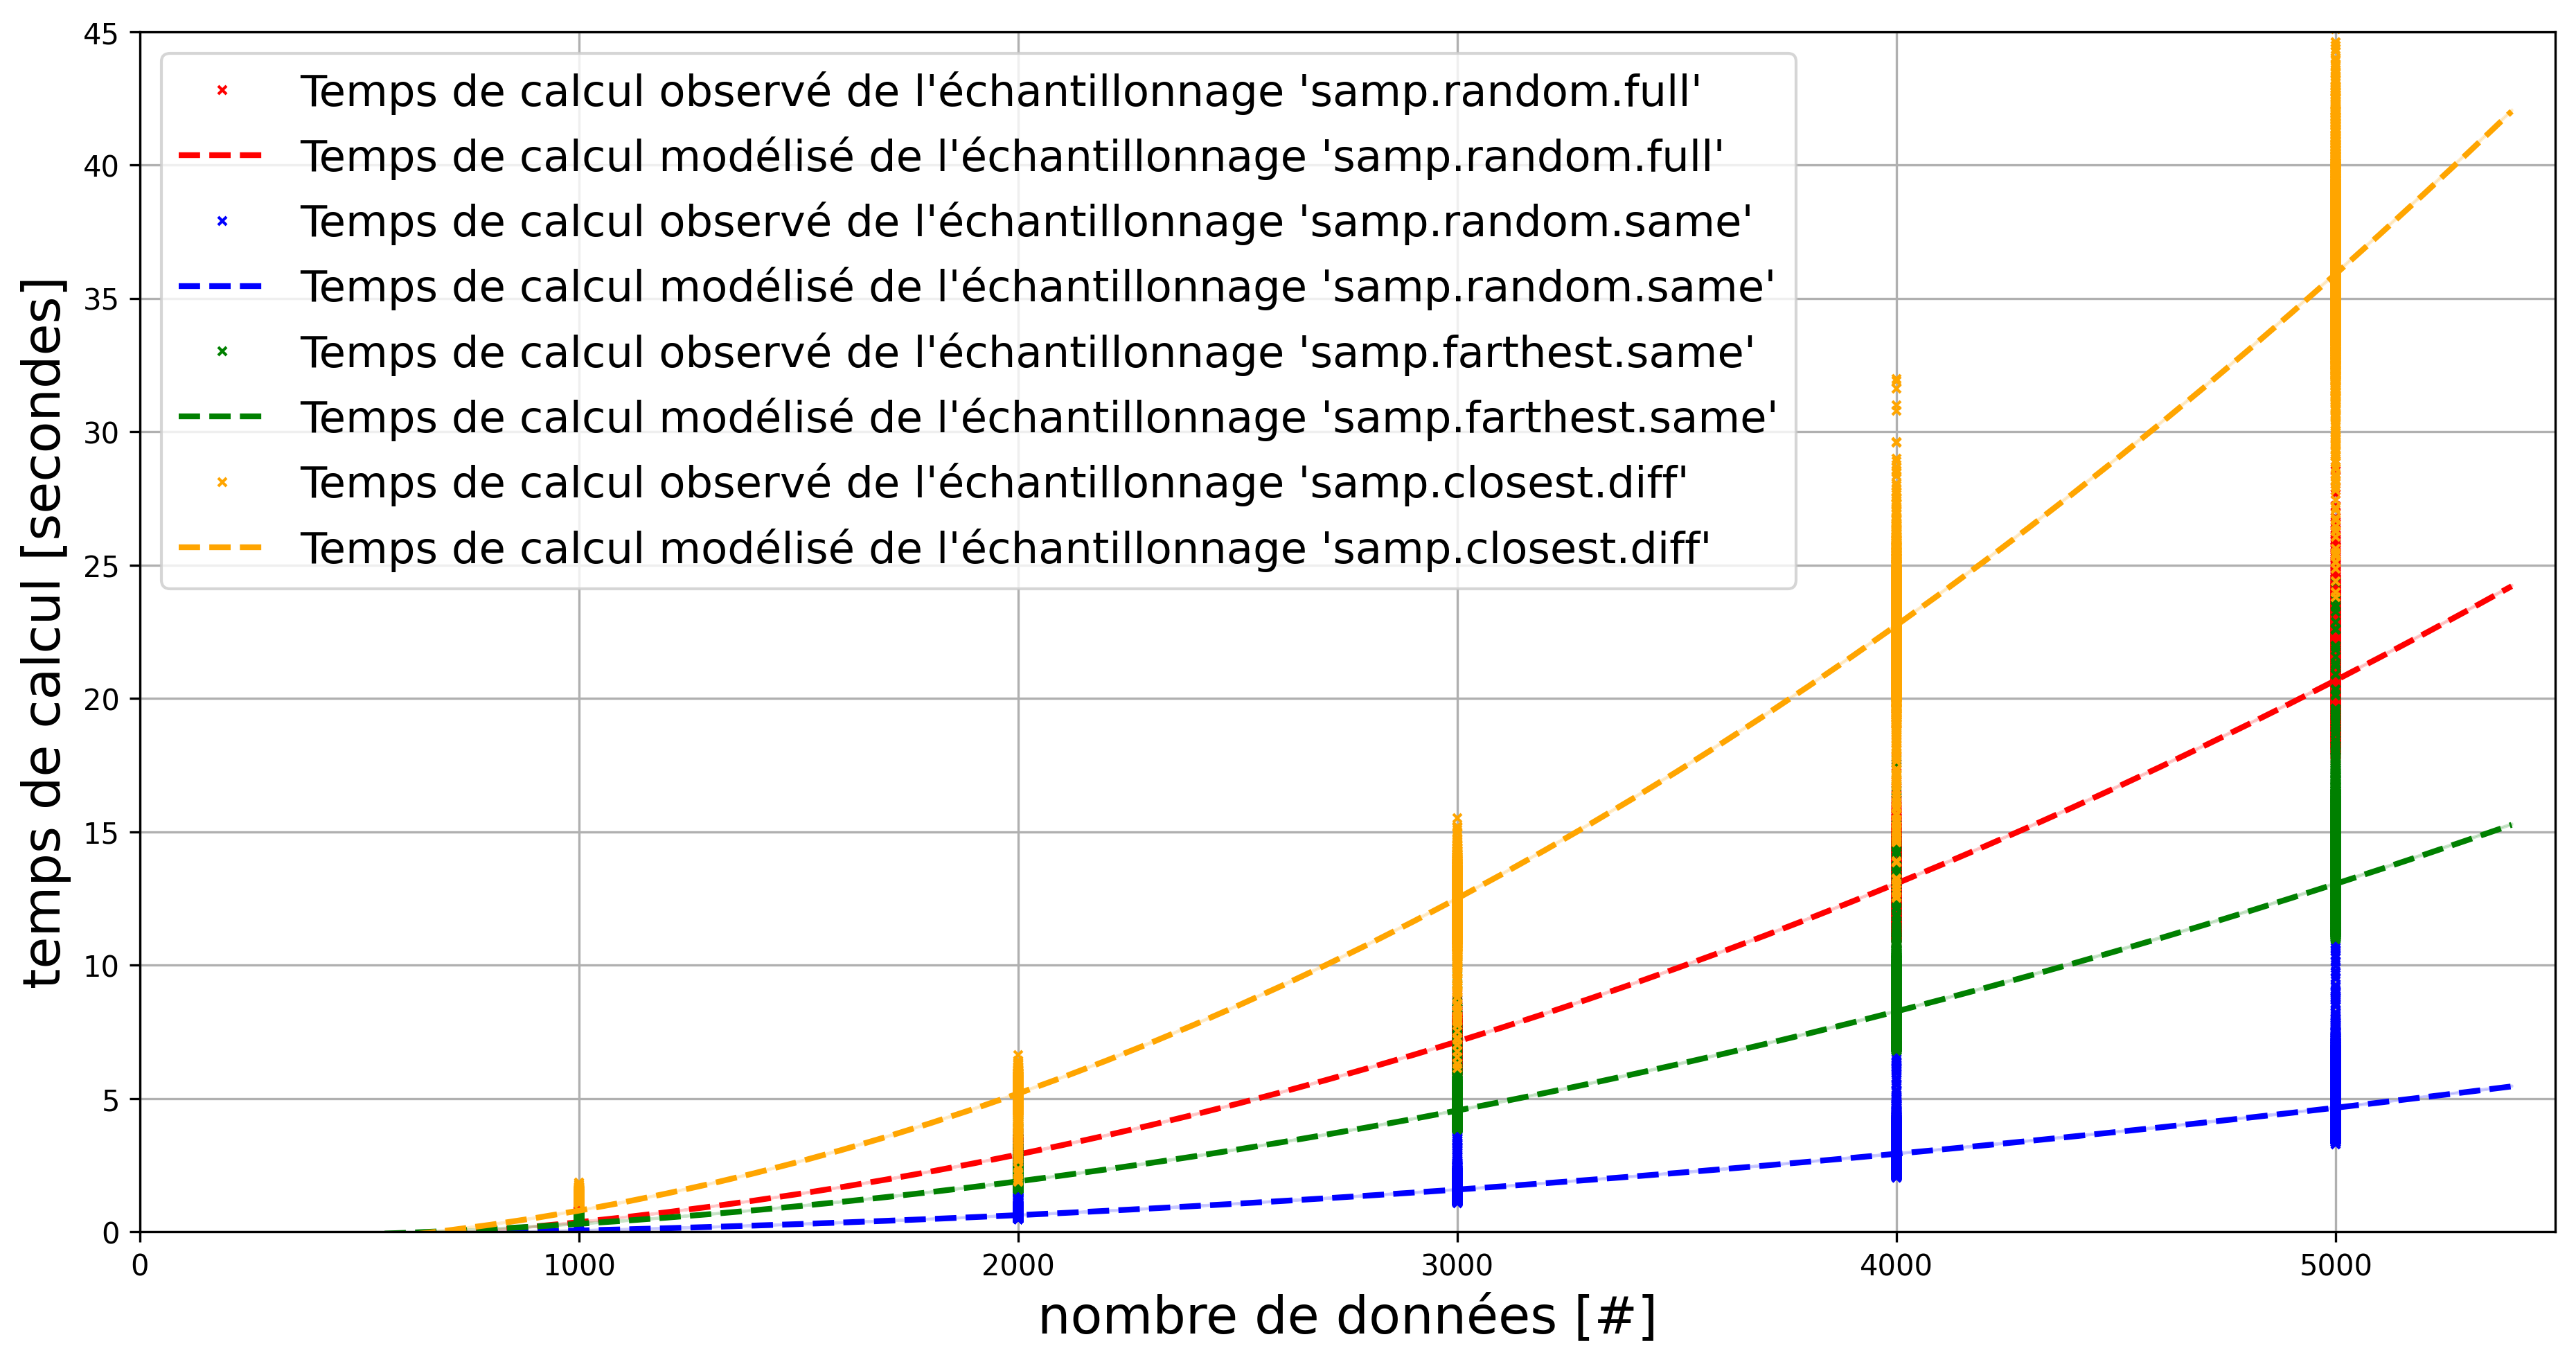
\includegraphics[width=0.8\textwidth]{figures/etude-temps-calcul-modelisation-4samp}
				\caption{Estimation du temps nécessaire (en secondes) pour effectuer une tâche d'\textbf{échantillonnage de contraintes} en fonction du nombre de données à traiter.}
				\label{figure:4.3.1-ETUDE-COUTS-TEMPS-CALCUL-MODELISATION-SAMPLING}
			\end{figure}

		%%% Discussion
		\subsubsection{Discussion}
		
			\todo[inline]{A REDIGER: Discussion}
	
	%%%
	%%% Subsection 4.3.2: Étude d'estimation du temps d'annotation par un expert métier
	%%%
	\subsection{Étude d'estimation du temps d'annotation par un expert métier}
	\label{section:4.3.2-ETUDE-COUTS-TEMPS-ANNOTATION}
	
		%%% Protocole expérimental.
		\subsubsection{Protocole expérimental}
		
			% Objectif de l'expérience.
			\todo[inline]{A REDIGER:}
			% Détails de l'expérience.
			\todo[inline]{A REDIGER:}
			% Description des tâches, des algorithmes et des paramètres.
			\todo[inline]{A REDIGER:}
			% Description de l'évaluation.
			\todo[inline]{A REDIGER:}
			% Pseudo-code.
			\todo[inline]{A REDIGER:}

			% Référence scripts.
			\begin{leftBarInformation}
				Les scripts de l'expérience (\textit{notebooks} Python) sont disponibles dans un dossier dédié de~\cite{schild:cognitivefactory-interactive-clustering-comparative-study:2021}.
			\end{leftBarInformation}

		%%% Résultats
		\subsubsection{Résultats obtenus}
		
			\todo[inline]{A REDIGER: Description figure}
			\begin{figure}[!htb]
				\centering
				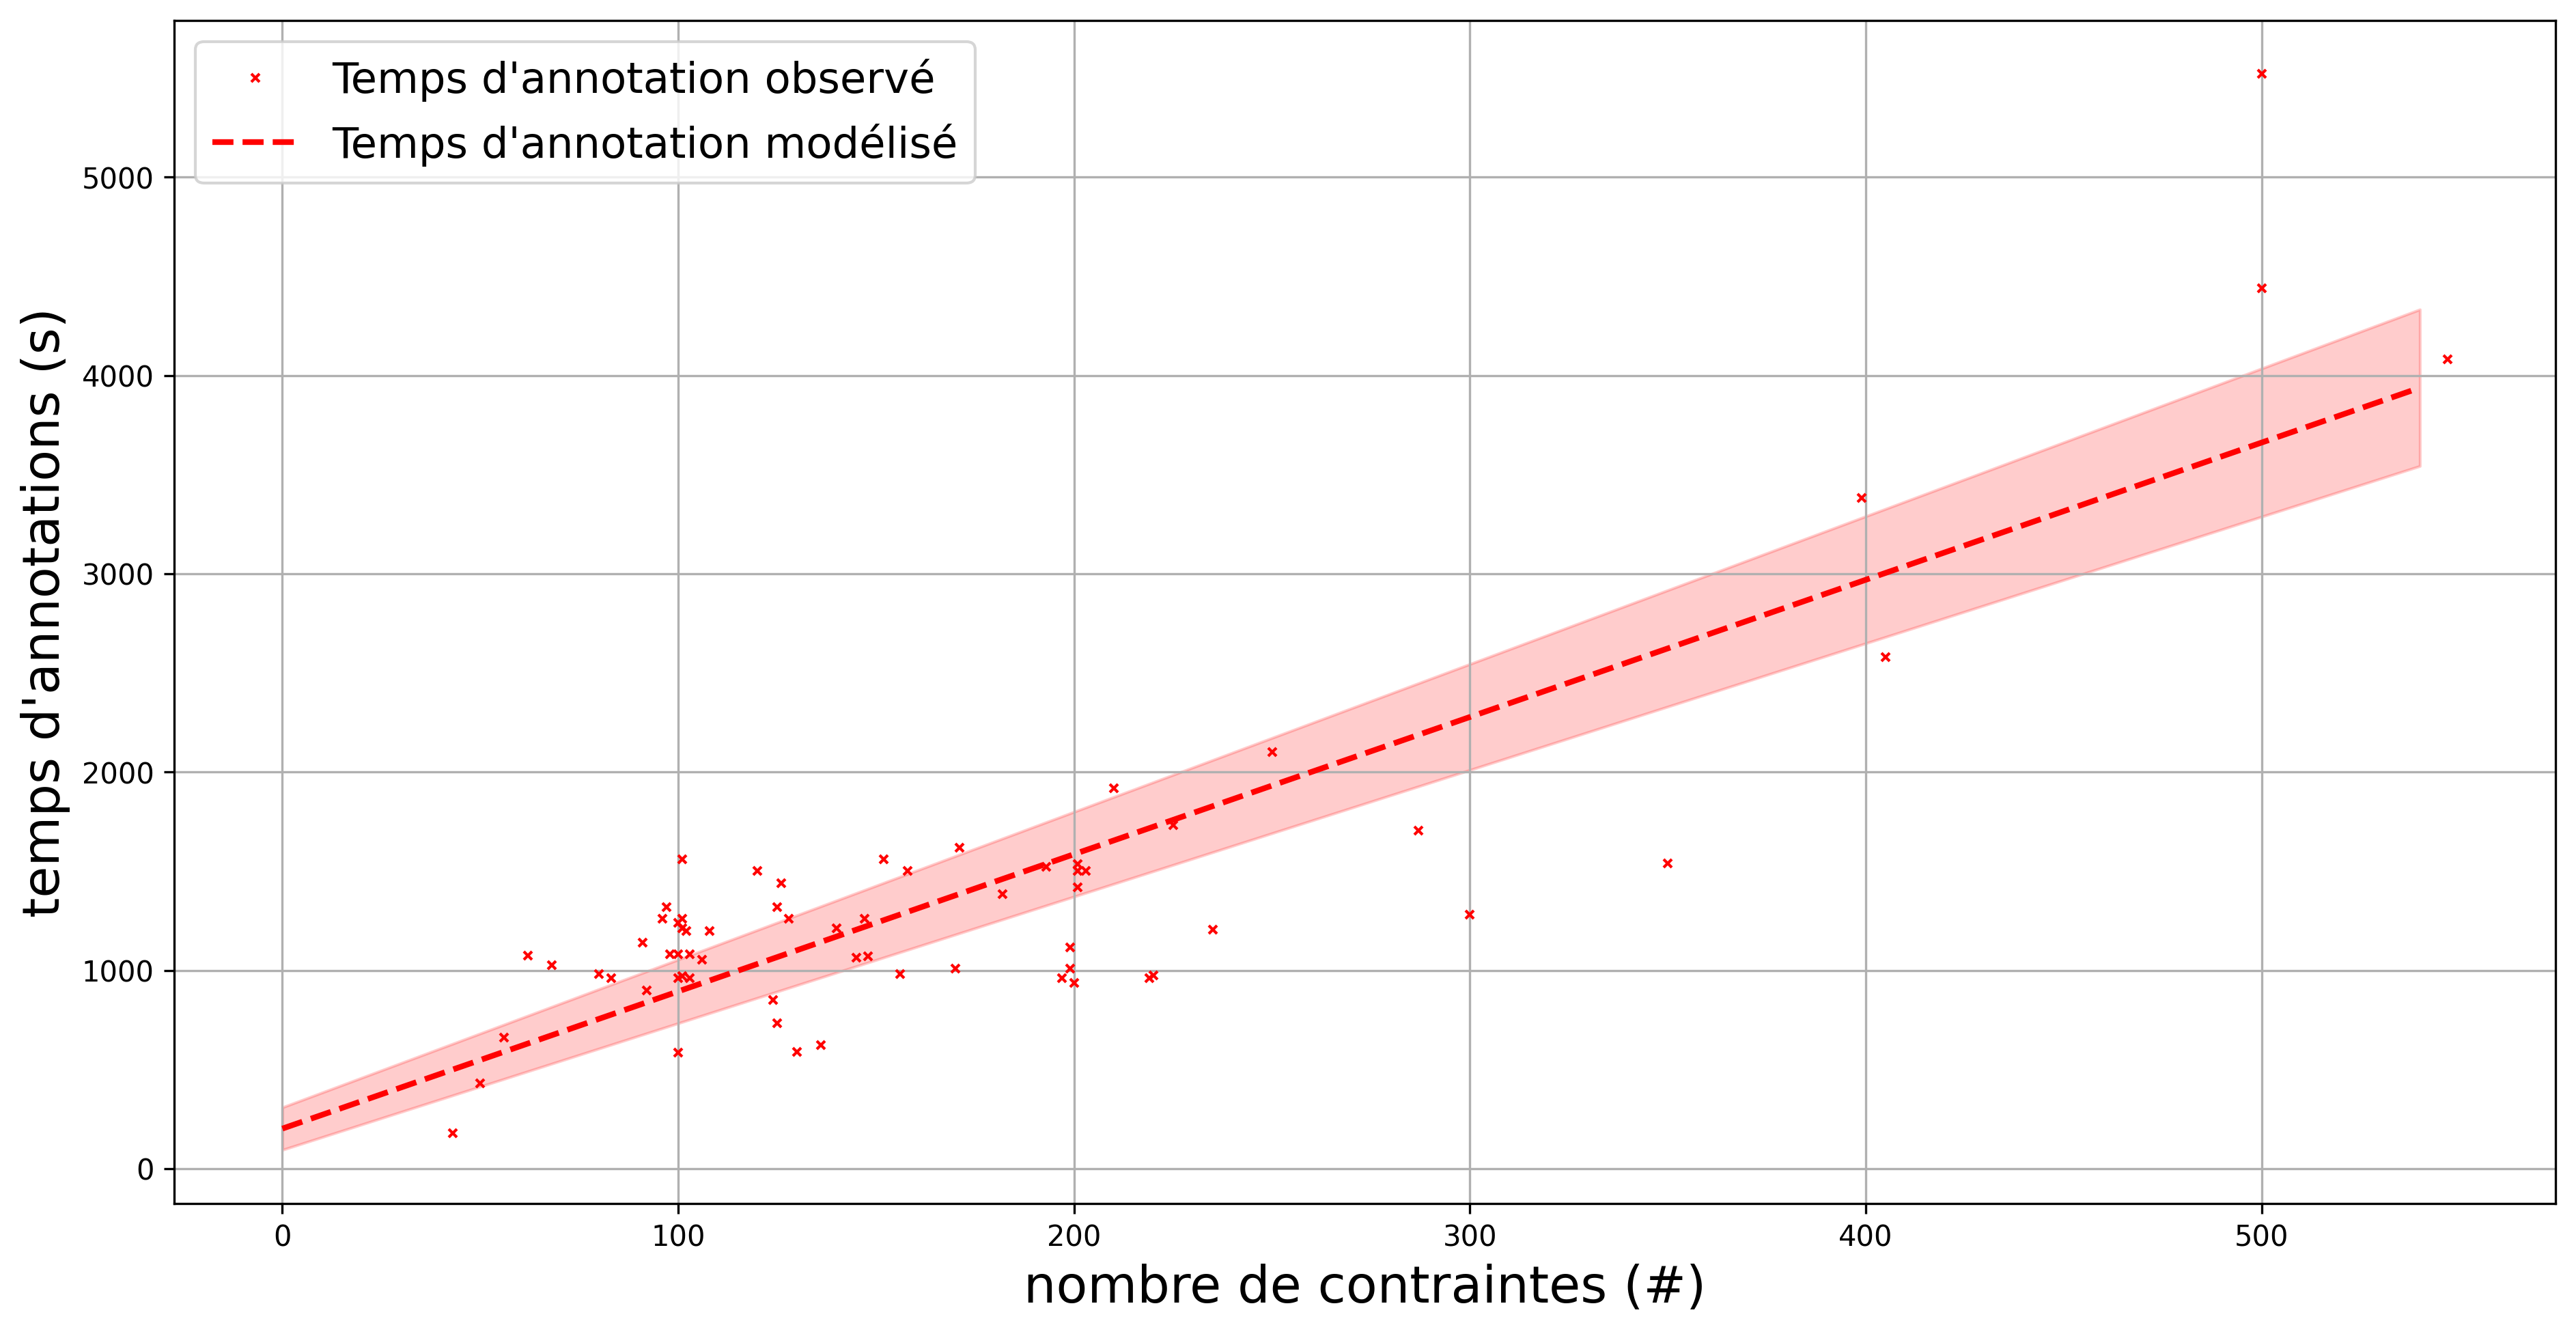
\includegraphics[width=\textwidth]{figures/etude-temps-annotation-1-modelisation-temps}
				\caption{Estimation du temps nécessaire (en secondes) pour annoter un lot de contraintes.}
				\label{figure:4.3.2-ETUDE-COUTS-TEMPS-ANNOTATION-SIMULATION}
			\end{figure}
			
			\todo[inline]{A REDIGER: quation du temps}
		
			\todo[inline]{A REDIGER: points plus gros ?}			
			\begin{figure}[!htb]
				\centering
				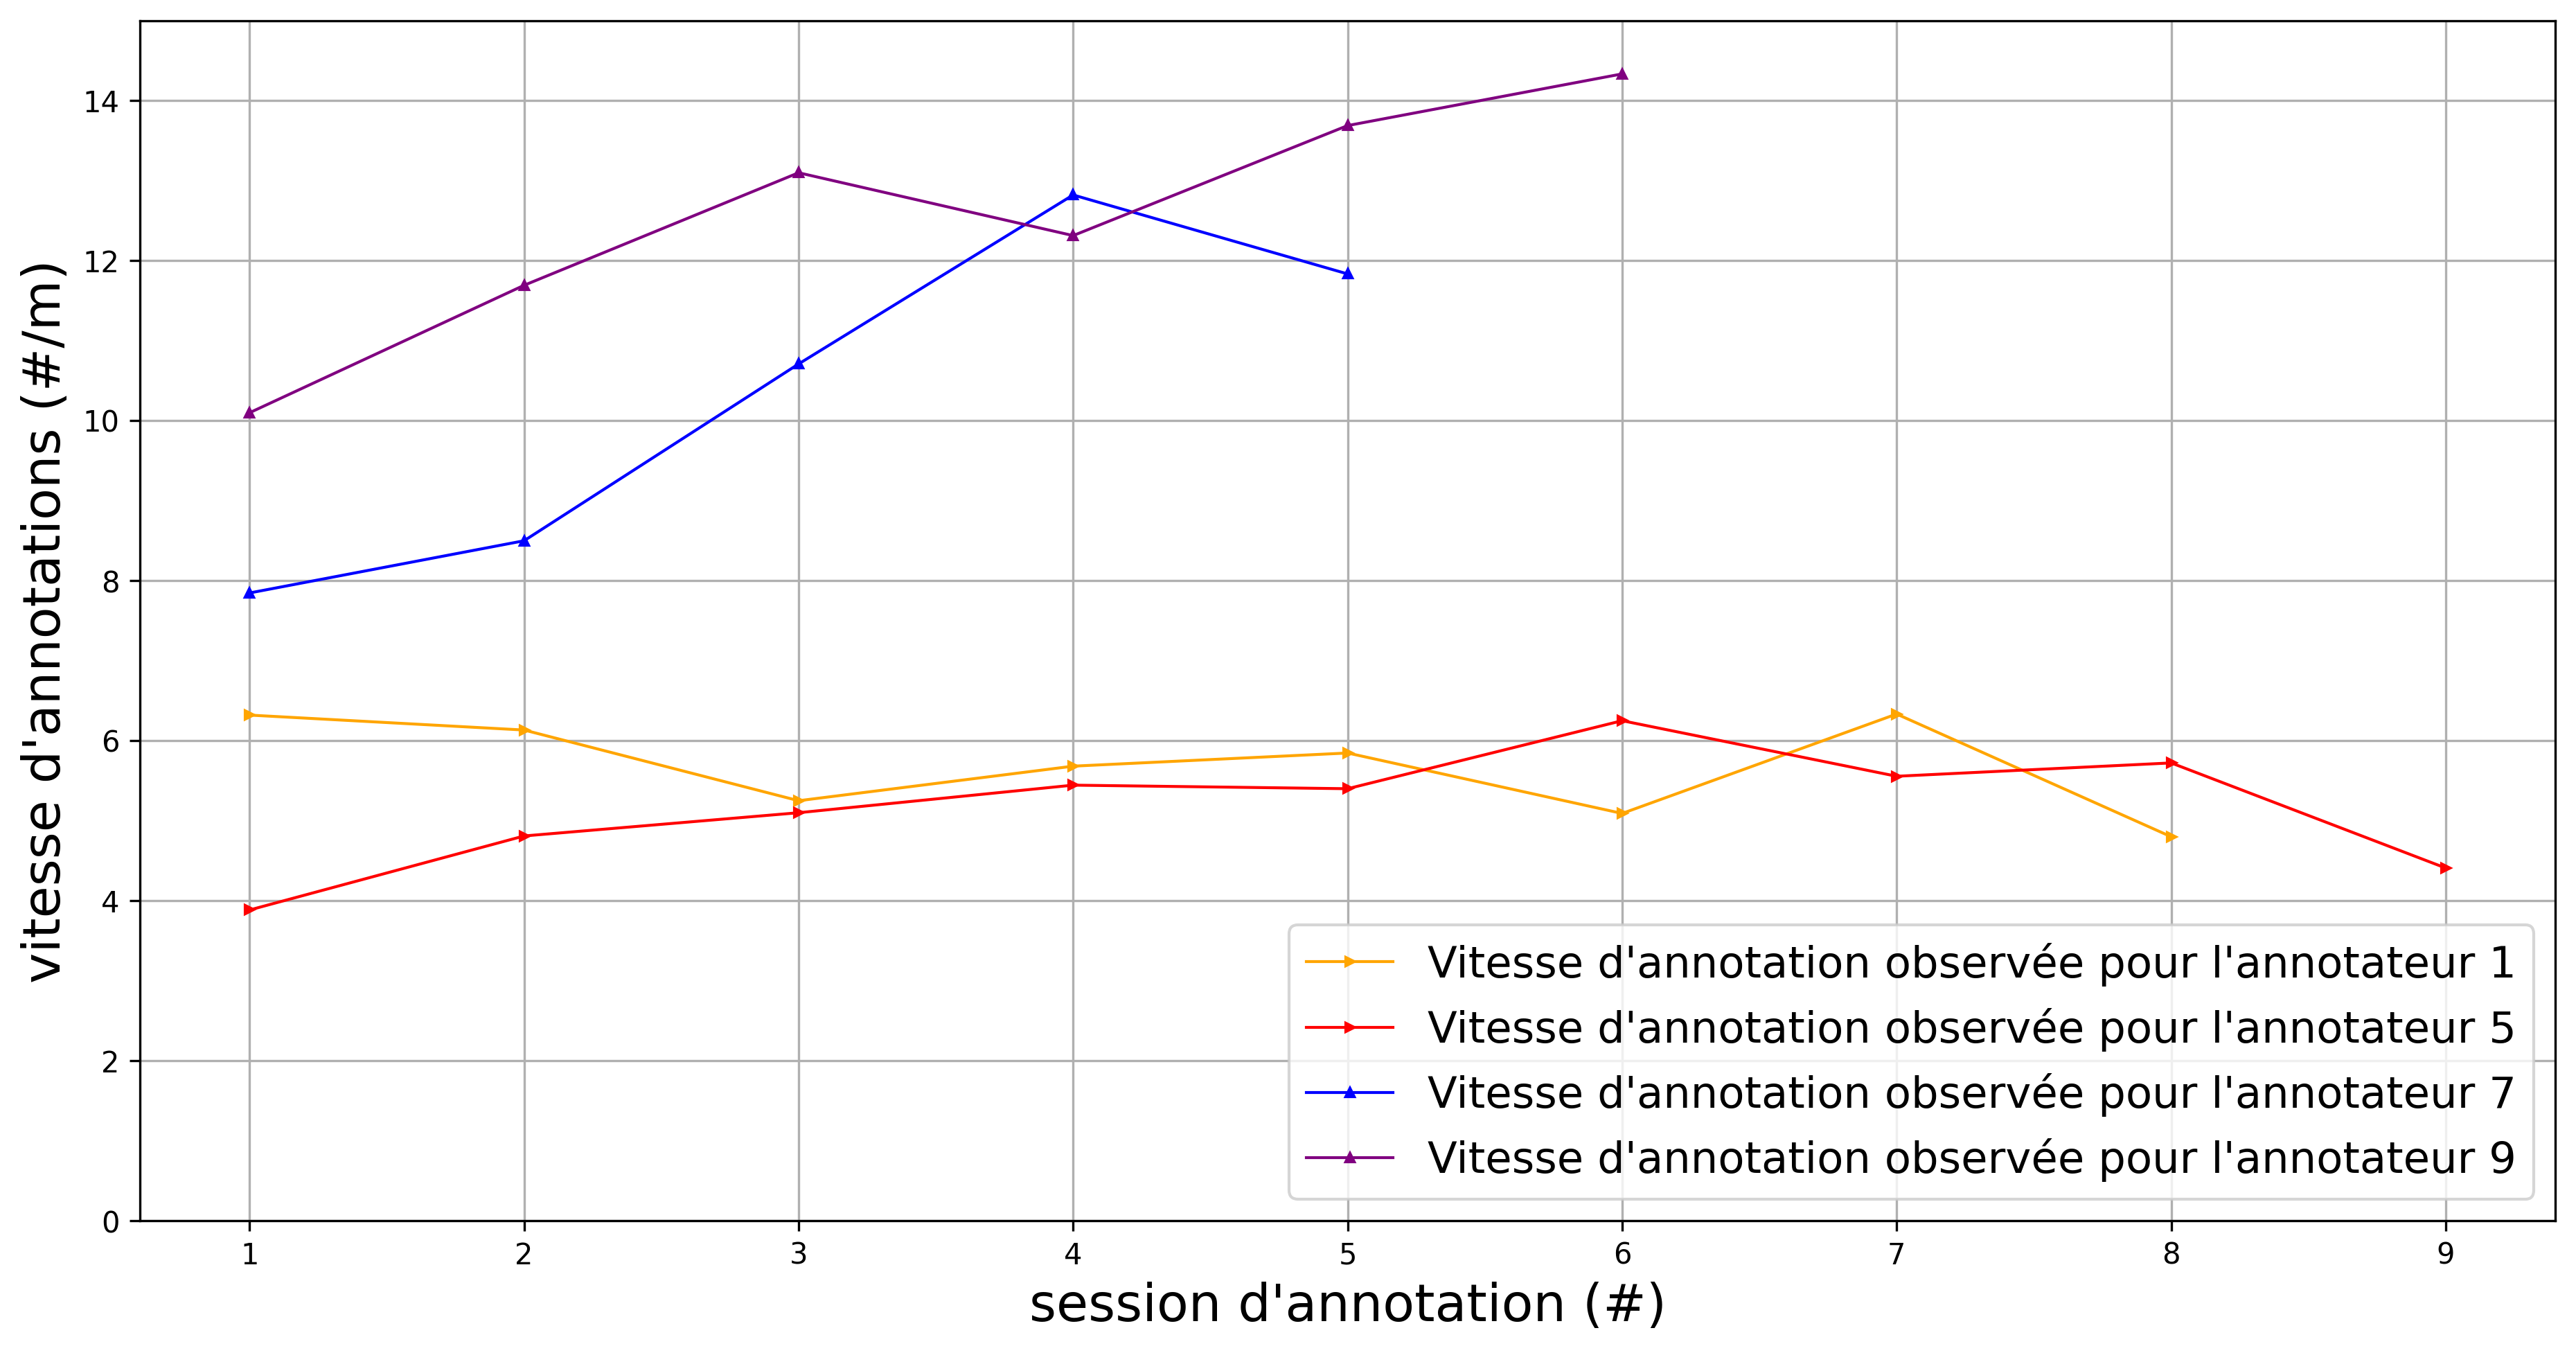
\includegraphics[width=\textwidth]{figures/etude-temps-annotation-3-etude-de-cas}
				\caption{Etude de cas d'évolution de la vitesse d'annotation de contraintes (en contraintes par minutes) en fonction des différentes sessions d'annotations}
				\label{figure:4.3.2-ETUDE-COUTS-TEMPS-ANNOTATION-EXEMPLE}
			\end{figure}

		%%% Discussion
		\subsubsection{Discussion}
		
			\todo[inline]{A REDIGER: Discussion temps moyen}
			\todo[inline]{A REDIGER: Discussion vitesse d'annotation}
	
	%%%
	%%% Subsection 4.3.3: Étude d'estimation du nombre de contraintes nécessaires
	%%%
	\subsection{Étude d'estimation du nombre de contraintes nécessaires}
	\label{section:4.3.3-ETUDE-COUT-NOMBRE-CONTRAINTES}
	
		%%% Protocole expérimental.
		\subsubsection{Protocole expérimental}

			% Objectif de l'expérience.
			\todo[inline]{A REDIGER:}
			% Détails de l'expérience.
			\todo[inline]{A REDIGER:}
			% Description des tâches, des algorithmes et des paramètres.
			\todo[inline]{A REDIGER:}
			% Description de l'évaluation.
			\todo[inline]{A REDIGER:}
			% Pseudo-code.
			\todo[inline]{A REDIGER:}

			% Référence scripts.
			\begin{leftBarInformation}
				Les scripts de l'expérience (\textit{notebooks} Python) sont disponibles dans un dossier dédié de~\cite{schild:cognitivefactory-interactive-clustering-comparative-study:2021}.
			\end{leftBarInformation}

		%%% Résultats
		\subsubsection{Résultats obtenus}

		%%% Discussion
		\subsubsection{Discussion}
	
	%%%
	%%% Subsection 4.3.4: Étude d'estimation du temps total d'un projet d'annotation
	%%%
	\subsection{Étude d'estimation du temps total d'un projet d'annotation}
	\label{section:4.3.4-ETUDE-COUTS-TOTAL}
	
		%%% Protocole expérimental.
		\subsubsection{Protocole expérimental}
		
			% Objectif de l'expérience.
			\todo[inline]{A REDIGER:}
			% Détails de l'expérience.
			\todo[inline]{A REDIGER:}
			% Description des tâches, des algorithmes et des paramètres.
			\todo[inline]{A REDIGER:}
			% Description de l'évaluation.
			\todo[inline]{A REDIGER:}
			% Pseudo-code.
			\todo[inline]{A REDIGER:}

			% Référence scripts.
			\begin{leftBarInformation}
				Les scripts de l'expérience (\textit{notebooks} Python) sont disponibles dans un dossier dédié de~\cite{schild:cognitivefactory-interactive-clustering-comparative-study:2021}.
			\end{leftBarInformation}

		%%% Résultats
		\subsubsection{Résultats obtenus}

		%%% Discussion
		\subsubsection{Discussion}